\def\mode{0}

\if 1\mode
    \documentclass[preprint,superscriptaddress,floatfix, nofootinbib]{revtex4-2}
%%CHINESE_PACKAGE_PLACEHOLDER%%

    \usepackage{lineno}
    \linenumbers
    \usepackage{natbib}
    \bibliographystyle{unsrt}
\else
    \documentclass[twocolumn,superscriptaddress, aps, prx,floatfix, nofootinbib]{revtex4-2}
%%CHINESE_PACKAGE_PLACEHOLDER%%

\fi

\usepackage{xcolor}
\usepackage{framed}
\definecolor{shadecolor}{RGB}{224,224,224}
\definecolor{orange(ryb)}{HTML}{FFA500}
\definecolor{lightorange(ryb)}{HTML}{FFB300}
\definecolor{dodgerblue}{HTML}{1E90FF}
\definecolor{lightdodgerblue}{HTML}{4dbff7}
\definecolor{crimson}{HTML}{FF4C4C}
\definecolor{pinkerton}{HTML}{e03185}
\definecolor{forest}{HTML}{6DD189}
\definecolor{lightishgray}{HTML}{DFDFDF}
\definecolor{error-red}{HTML}{EFB2B6}

\usepackage{dsfont}
\usepackage{graphicx}
\usepackage{dcolumn}
\usepackage{bm}
\usepackage{float}
\usepackage{siunitx}
\usepackage{braket}
\usepackage{amsmath,amssymb}
\sisetup{uncertainty-mode=separate}
\usepackage[
	pdftex,
	colorlinks=true,
  	urlcolor=dodgerblue,
  	linkcolor=dodgerblue,
  	citecolor=dodgerblue
]{hyperref}

\usepackage{ulem}
\begin{document}

\title{哈伯德量子模拟器中的拓扑相变与混合态序}
\author{
Lin~Su$^{*,\dagger,1}$,
Rahul~Sahay$^{*,1}$,
Michal~Szurek$^{1}$,
Alexander~Douglas$^{1}$,
Ognjen~Markovi\'{c}$^{1}$,
Ceren~B.~Dag$^{\S, 1,2,3}$,
Ruben~Verresen$^{4}$,
and Markus~Greiner$^{\ddagger,}$
}

\affiliation{
Department of Physics, Harvard University, Cambridge, Massachusetts 02138, USA\\
$^2$Department of Physics, Indiana University, Bloomington, Indiana 47405, USA\\
$^3$ITAMP, Harvard-Smithsonian Center for Astrophysics, Cambridge, MA 02138, USA\\
$^4$Pritzker School of Molecular Engineering, University of Chicago, Chicago, IL 60637, USA\\
$^*$These authors contributed equally, $^\dagger$ls4211@columbia.edu,
$^\S$cbdag@iu.edu,
$^\ddagger$greiner@physics.harvard.edu
}

\date{\today}
\begin{abstract}
拓扑相变通过区分局域不可分辨而全局迥异的物相,对多体物理的传统范式提出了挑战。我们利用光晶格中相互作用的铒原子量子模拟器,观测到一维晶体对称性保护拓扑相(CSPT)之间的这类转变。通过非局域弦序参量检测临界点,并揭示其与莫特绝缘体-霍尔丹绝缘体相变预测的关联性。更引人注目的是,我们证实了两个相同系统堆叠会消除相变,验证了SPT相可逆性的群结构预测。此外,虽然引入对称性破缺无序也会消除相变,但通过无序平均可使其重现。因此,相邻物相实现了一种混合态量子序——其间的临界性取决于观测者的信息。我们的研究结果揭示了拓扑与信息如何影响量子相变,为探索可编程量子物质中的新型临界现象开启了大门。
\end{abstract}

\maketitle
\section{引言}

\begin{figure*}
    \centering
    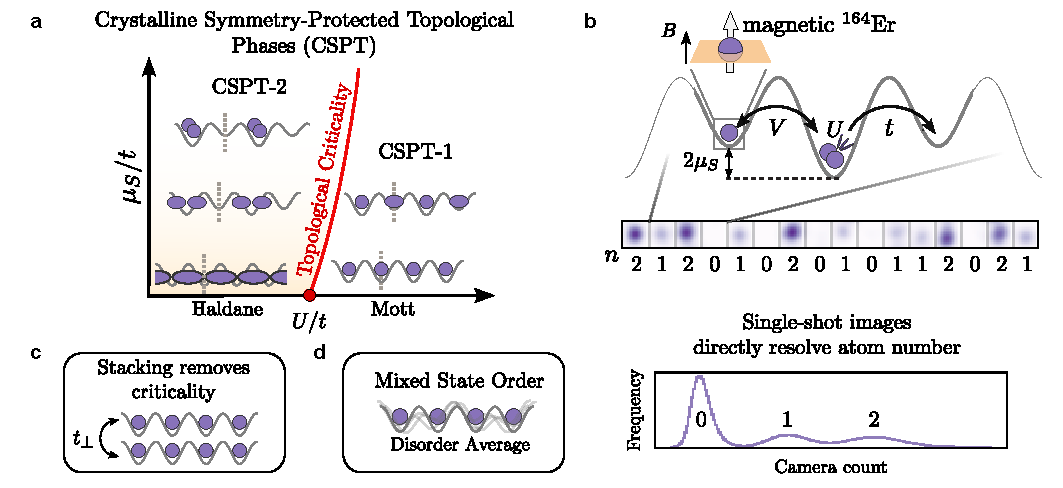
\includegraphics[width=\textwidth]{figures/Fig_intro_v4.pdf}
    \caption{\textbf{交错偶极玻色-哈伯德量子模拟器中的拓扑相与临界性。}
    \textbf{a},在长程密度-密度相互作用($V$)下,一维扩展玻色-哈伯德相图\cite{Torre2006, Berg2008}中涌现出受对称性保护的拓扑(SPT)相——Haldane绝缘体(HI)。该相与Mott绝缘体(MI)属于不同物相。值得注意的是,当引入交错化学势$\mu_S$时,拓扑相变依然存在。在此机制下,HI与MI表现为两种不同的晶体SPT(CSPT)原子极限,其拓扑保护源于玻色子宇称守恒(公式\eqref{eq: parity-generator})与位点中心反演对称性(虚线标示)\cite{Fuji2015}。
    \textbf{b},实验中我们通过光晶格中的$^{164}$Er玻色原子实现该模型。粒子以振幅$t$隧穿,并感受强度为$U$的局域相互作用。铒原子间的偶极相互作用诱导了最近邻强度为$V$的长程密度-密度耦合。超晶格产生交错化学势$\mu_S$。我们直接解析了每个位点的原子数而无须宇称投影。图示为代表性单次拍摄图像,下方标注数字化占据数。相机计数直方图显示每个位点存在$0$、$1$和$2$粒子的峰。
    \textbf{c},我们通过堆叠两个一维链实例来探究拓扑临界态的稳定性,证明这些量子物相具有可逆性。
    \textbf{d},进一步研究表明,临界态对可编程对称性破缺无序敏感,但通过无序平均可恢复其稳定性。在此意义上,这些SPT对应着不同的混合态量子物相~\cite{Ma2023}。
    }
    \label{fig: setup}
\end{figure*}

处于平衡态的多粒子相互作用体系会发生宏观性质突变的相变现象~\cite{Sachdev1999}。传统上,这类相变由朗道范式描述,该理论认为当局部可观测量(或"序参量")的关联呈现长程特性并自发破缺系统对称性时,相变随即发生。该理论成功解释了诸多有限温度下的相变,如液体与晶体间的转变,或不同类型磁体间的转变。然而在接近绝对零度时,量子效应会导致"拓扑"相变——这类相变没有对应的温度驱动版本,其相区分依赖于非局域量子关联而非局部测量。

值得注意的是,这类拓扑相变甚至在一维量子系统中也被预言存在,即对称性保护拓扑(SPT)相之间的转变~\cite{Senthil2015, Pollmann2010, Turner11, Fidkowski11, Pollmann2012, Schuch2011, Chen2011, Chen2012}。近年来,类比量子模拟技术的进步使得一维SPT相的实现成为可能——实验平台涵盖超冷原子~\cite{Atala2013, Meier2016, Sylvain2019, Sompet2022}、超导电路~\cite{Cai2019}和囚禁离子~\cite{Katz2024}等体系,此外还包括数字量子模拟\cite{Choo2018, Smith2022, Herrmann2022}。然而,在类比模拟器中探测这些相之间的量子临界点仍面临重大挑战,需要可调参数来扫描整个相变过程。

本工作中,我们在类比量子模拟器中实现了SPT相之间的量子临界点(图~\ref{fig: setup}a),并通过研究其在堆叠和无序条件下的稳定性与失稳性来证实其拓扑本质(图~\ref{fig: setup}c, d)。我们采用量子模拟器\cite{Bloch2008, Gross2017, Bohrdt2021}实现具有长程相互作用和交错化学势的玻色-哈伯德模型变体(图~\ref{fig: setup}b):
\begin{equation}
\label{eq: Hamiltonian}
\begin{split}
H=-t\sum_{x}(\hat{a}_x^\dag \hat{a}_{x + 1}+\mathrm{h.c.})+\frac{U}{2}\sum_x\hat{n}_x(\hat{n}_x-1) \\
+\sum_{x, r>0}V_{r}\hat{n}_x\hat{n}_{x + r} - \mu_S\sum_x(-1)^x\hat{n}_x.
\end{split}
\end{equation}
其中$t$、$U$和$\mu_S$分别表示隧穿强度、在位相互作用和交错势强度;$a_x^{\dagger}$($a_x$)在$x$位点产生(湮灭)一个玻色子,$\hat{n}_x = a_x^{\dagger} a_x$为粒子数算符。$V_r$描述距离$r$处的长程偶极相互作用(见补充材料SM)。我们将该模型称为交错偶极玻色-哈伯德模型。前期工作\cite{Torre2006,Berg2008}曾预言其相图中存在Haldane绝缘体\cite{Haldane1983},我们亦对此进行了探究。

为实现该哈密顿量模拟,我们采用具有偶极相互作用的磁性铒原子~\cite{Su2023},并通过Fano-Feshbach共振调节在位相互作用~\cite{Chin2010}(图~\ref{fig: setup}b)。我们将玻色性$^{164}$Er原子绝热装载至二维光晶格中,通过单方向强约束形成孤立的一维链(SM)。经过数千次实验重复后,采用包含限制单元填充样本分析的数据筛选流程(SM),边界条件详见SM。最终通过位点分辨成像~\cite{Bakr2010, Sherson2010}获得无需宇称投影的原子数测量结果~\cite{Su2024}。
\section{晶体对称性保护的拓扑相及其相变} \label{sec:CSPT-transitions}
\begin{figure*}
    \centering
    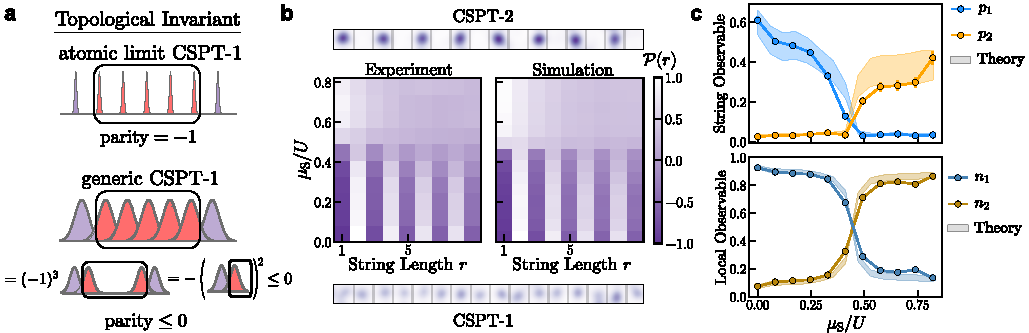
\includegraphics[width=\textwidth]{figures/Fig_CSPT_ground.pdf}
    \caption{\textbf{晶体对称性保护拓扑相之间的量子相变。}我们研究了16个位点一维链中两种CSPT之间的量子相变。\textbf{a},对于原子极限CSPT,单位填充态下奇数长度弦的宇称具有$-1$奇偶性。即使量子涨落(例如由隧穿效应引起)使系统偏离该原子极限态且玻色子轻微离域化,在位点中心反演对称性存在时,宇称仍保持负值。\textbf{b},奇数长度弦宇称的符号可区分两种CSPT并提供一个拓扑不变量。当$\mu_S$跨越量子临界点时,系统从CSPT-1相(类莫特绝缘体,底部)过渡到CSPT-2相(类电荷密度波,顶部)。我们实验测量的弦宇称与考虑读取保真度的模拟结果(SM)高度吻合。\textbf{c},我们利用弦宇称测量定义了CSPT-1和2的两个有效"弦序参量"($p_1$和$p_2$),如顶部面板所示。实验观测值以误差棒(自助法标准误差)表示,并与模拟结果(本文所有阴影区域均表示95\%置信区间)进行对比。在相变的CSPT-1侧,$p_2$观测量(橙色)实际为零(受限于有限成像保真度),而局域平均密度观测量$n_2$(棕色)显著非零,凸显了CSPT的拓扑特性。这表明局域观测量无法区分两种CSPT,而宇称"弦序参量"可以。局域观测量的交叉现象并非源于有限尺寸效应(SM)。}
    \label{fig: CSPT_ground}
\end{figure*}
我们首先阐述保护SPT相及其相变的两种对称性。第一,由于粒子数守恒,系统保持链中玻色子总数的\textit{宇称}(偶数或奇数性)。这产生了由以下生成元决定的哈密顿量$\mathbb{Z}_2$对称性:
\begin{equation} \label{eq: parity-generator}
 \hat{\mathcal{P}} = \prod_{x} e^{i \pi \hat{n}_x}   .
\end{equation}
此外,该模型还表现出位点中心反演对称性$\hat{\mathcal I}$:这是一种\textit{晶体}对称性,可将晶格关于给定位点进行反演。我们所研究的拓扑相受此晶体对称性以及内禀宇称对称性的保护,因此可称为晶体对称性保护的拓扑相(CSPTs)\cite{Fu11, Turner10inversion, Hughes11, Fuji2015, Song17}。

这些相出现在系统相图中单位填充$\bar{n} =1$且昂萨格 Hubbard相互作用远大于隧穿强度的参数区域,如图~\ref{fig: setup}a相图上部所示。第一个CSPT相(CSPT-$1$)本质上是莫特绝缘体,出现在交错化学势较小的情况下。此时强昂萨格 Hubbard相互作用使得每个位点的平均玻色子数稳定在$1$附近。相反,第二个CSPT相(CSPT-$2$)出现在交错化学势较大时,此时奇数位点上平均占据两个玻色子("双粒子态")而偶数位点没有玻色子。这些构型示意性地展示在图~\ref{fig: setup}a的相图中,其中经典态($\ket{1111\cdots}$和$\ket{2020\cdots}$)在原子极限(即隧穿强度$t\to 0$时)成为精确解。在存在前述宇称$\hat{\mathcal P}$和反演$\hat{\mathcal I}$对称性的情况下,这两个态无法绝热连接~\cite{Fuji2015}。事实上,虽然量子涨落存在时无法用局域序参量区分这两个相\cite{Fuji2015},但它们可通过非局域拓扑不变量加以区分。该不变量正是奇数长度大区域内玻色子宇称的\textit{符号}。具体而言,该符号在CSPT-1中为负(CSPT-2中为正),且不关闭能隙就无法改变(图~\ref{fig: CSPT_ground}a及补充材料)。
\begin{figure*}
    \centering
    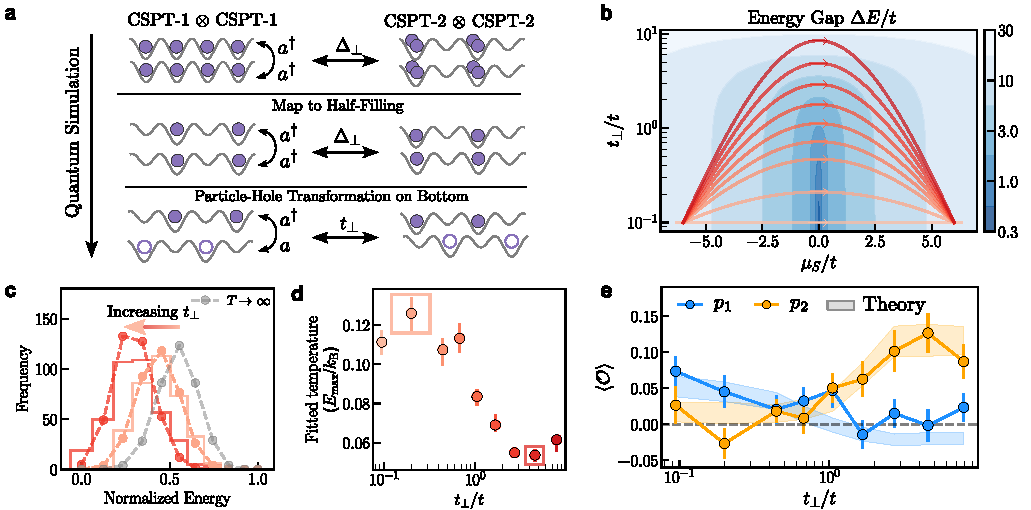
\includegraphics[width=\textwidth]{figures/Fig_stacking.pdf}
    \caption{\textbf{通过堆叠消除相变。}耦合偶数条$\mathbb{Z}_2$拓扑链可使拓扑性平庸化。\textbf{a},为量子模拟方程~\eqref{eq: coupling}中的对产生耦合,我们将模型(顶行)映射至半填充表示(中行),再对底链进行粒子-空穴变换(底行)。系统尺寸为2×10个格点。\textbf{b},当链间隧穿$t_\perp$非零时,单条CSPT链临界点(如$\mu_S/t = 0$处)的数值计算能隙变为有限值。为探测该能隙,我们在最小$t_\perp$下初始化两条CSPT-1链,并通过不同中间值过渡至CSPT-2区域。随时间线性改变交错化学势$\mu_S$,同时将$t_\perp$调节至最终可忽略耦合的构型,并读取演化态的瞬时快照。\textbf{c},在最终$\mu_S = 6t$点处隧穿可忽略,态密度可用经典方法近似。通过分析各快照计算末态能量直方图。随着$t_\perp$增大,提取的温度降低。彩色柱为实验数据;彩色虚线为吉布斯分布拟合;灰色虚线显示无限温度分布。\textbf{d},实测温度(误差棒:自助法68\%置信区间)随$t_\perp$增大系统性下降。\textbf{e},最大$t_\perp$对应的宇称序参量(误差棒:自助法标准误)揭示仅当耦合足够强时才出现向CSPT-2相的交叉转变,这与存在带隙路径的结论一致。}
    \label{fig: Coupled_CSPT}
\end{figure*}

为在量子模拟器中演示这两个不同的拓扑相,我们通过定义如下的宇称"弦算符"实验测量\cite{Hilker17, Wei23}该拓扑不变量:
\begin{equation}
\label{eq: POP}
\mathcal{P}_{x_0}(r) =  \left\langle \prod_{x=x_0}^{x_0+r} e^{i\pi \hat n_x}\right\rangle \equiv \langle \hat{\mathcal{P}}_{x_0}(r) \rangle,
\end{equation}
该算符精确测量区域内玻色子的平均宇称。实验结果如图~\ref{fig: CSPT_ground}b所示,作为交错场与相互作用强度之比$\mu_S/U$的函数。正如预期,对于弱交错场,奇数长度弦的宇称为负(反映拓扑不变量),而偶数长度弦的宇称为正;对于强交错场,所有弦长度的宇称均为正。这些观测结果与数值模拟一致(见补充材料)。

通过计算交错与均匀宇称"弦序参量"$p_1$和$p_2$可以诊断这些相的显著区别,二者分别定义为对足够长$r$取平均的$(-1)^{r} \mathcal{P}_{x_0}(r)$和$\mathcal{P}_{x_0}(r)$(见补充材料)。如图~\ref{fig: CSPT_ground}c顶部面板所示,这些序参量能清晰区分两相:在各自相中取有限值或零值,并在临界点处呈现急剧转变。论证这些序参量在相应相外消失的一种方法是利用该模型在三粒子态缺失区域中的近似粒子-空穴对称性(见补充材料)。
相比之下,我们还定义了平均密度涨落的局域观测量:$n_2= \langle (-1)^i\delta\hat{n}_i\rangle $(其中$\delta \hat{n}_i=\hat{n}_i-1$)以及$n_1= 1 - n_2$(图~\ref{fig: CSPT_ground}c 底部)。这些观测量在相变过程中的平滑变化反映了局域观测量无法准确区分两个相态的特征——这正是拓扑相的定义性特征(参见补充材料)。这些观测结果强有力地支持了在$\mu_S \ll U$和$\mu_S \gg U$处存在两个截然不同的CSPT相,且它们被一个量子相变所分隔,这与我们的大规模基态数值模拟结果一致~\cite{Sahay2025}(补充材料)。
\section{耦合偶数条链可消除拓扑相变}

在识别出CSPT相之间的量子相变后,我们现通过利用SPT相的一个关键性质来展示如何消除这一相变。即通过堆叠并耦合一定数量的相同链,可使整体状态变为拓扑平庸态\cite{Turner11, Fidkowski11, Pollmann2012, Schuch2011, Chen2011, Chen2012}。这允许在不同相之间建立连续、有能隙的路径——从而消除中间的量子临界点。该性质与对称破缺相形成鲜明对比,后者在多重堆叠后仍保持对称破缺特性,因此无法与对称性保持态连续连通。

我们通过向方程~\eqref{eq: Hamiltonian}的双链版本添加如下配对项来探究这一堆叠性质:
\begin{equation}
    H_{\perp} = \Delta_{\perp} \sum_{x} a^{\dagger}_{\mathsf{T}, x} a^{\dagger}_{\mathsf{B}, x}   + \text{h.c.},
\label{eq: coupling}
\end{equation}
该操作在两组CSPT-1与CSPT-2相的堆叠之间建立了有能隙的路径(图~\ref{fig: Coupled_CSPT}a顶部)。此处$a_{x, \mathsf{T}/\mathsf{B}}^{(\dagger)}$标记顶/底层的玻色湮灭(产生)算符。关键的是,上述项保留了由方程~\eqref{eq: parity-generator}生成的保护性$\mathbb{Z}_2$宇称对称性,以及位点中心反演对称性。

我们采用粒子-空穴映射模拟该配对项,如图~\ref{fig: Coupled_CSPT}a所示并在补充材料中详述。从两条链均处于$t_\perp$可忽略的深度CSPT-1态出发,我们跨越单条CSPT链的临界点$\mu_S=0$,进入每条解耦链的基态均为CSPT-2态的成像前区域。图~\ref{fig: Coupled_CSPT}b的数值等高图显示,随着链间$t_\perp$增大,$\mu_S=0$处基态与第一激发态间的多体能隙增大,消除了量子临界性。$\mu_S$与$t_\perp$的斜坡遵循不同阴影的红色线条,其中$\mu_S$斜坡保持恒定速率。

在低链间隧穿$t_\perp \rightarrow 0$时,斜坡无法在跨越量子临界点的零能隙处保持绝热性。系统因此升温,导致末态相对于CSPT-2基态的保真度降低。这通过CSPT-2序参量$p_2$的测量得以揭示(图~\ref{fig: Coupled_CSPT}e),其值在$t_{\perp}$较小时远低于基态期望值。类似地,CSPT-1序参量在此区域也不会消失。相比之下,在较大$t_\perp$值时,尽管相图中路径总长增加(因需在相同总扫描时间内同步改变$t_\perp$与$\mu_S$),我们仍观察到更精确的CSPT-2态制备,这体现为其序参量值的增大。
\begin{figure*}
    \centering
    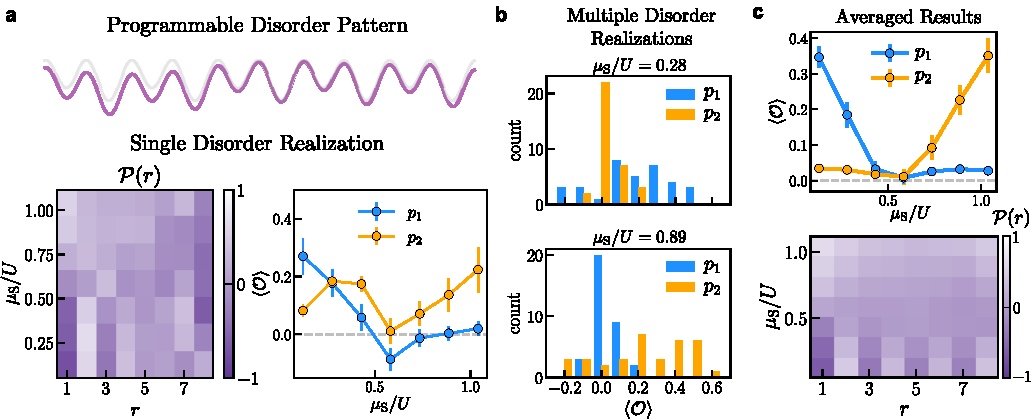
\includegraphics[width=\textwidth]{figures/CSPT_average.pdf}
    \caption{\textbf{局域无序导致的混合态CSPT。} \textbf{a},为证明位点中心对称性对保护CSPT的重要性,我们刻意引入可编程化学势无序(原浅灰色晶格变为紫色晶格)。下图显示单次化学势无序实现的序参量(自助法标准误差)不再呈现清晰分明的物相。左下图展示了不同交错势下的空间序分布,右下图则通过空间积分绘制弦序参量。\textbf{b},不同无序实现中$p_1$和$p_2$的分布直方图表明,无序会导致各实现中序参量的强烈畸变。\textbf{c},由于CSPT受平均对称性保护,通过对不同无序实现取平均后,我们从上图序参量中获得了两个明确区分的混合态物相信号(均值标准误差)。受有限成像保真度、有限尺寸效应及粒子-空穴对称性近似程度影响(详见补充材料),序参量虽未精确归零但仍可区分两相。底图显示拓扑不变量正是奇数长度宇称弦的平均值符号——大$\mu_S$时为正,小$\mu_S$时为负。}
    \label{fig: CSPT_average}
\end{figure*}

更大的能隙允许我们以更少热效应跨越相图,这也反映在所制备CSPT-2态的最终温度上(图~\ref{fig: Coupled_CSPT}c)。由于在读取阶段链内隧穿($t$)远小于其他能量尺度($\mu_S$、$U$和$V$),末态能量可很好地用经典态能量近似。基于每个快照,我们计算末态能量并获得态分布的直方图。通过拟合温度参数,可观察到随着$t_\perp$增大,温度向低温区移动。

这为$\mathbb{Z}_2$拓扑相中耦合两条CSPT链会打开能隙并消除量子临界点的理论预测~\cite{Gu2009}提供了实验证据。同时验证了SPT相的"可逆性"~\cite{Freed2014}——这一特征将其与非可逆相(如对称破缺序或本征拓扑序)区分开来。
\section{混合态序与平均对称性}

至此,我们已在实验中证实了两种不同CSPT相的存在,并展示了它们之间相变的一个标志性特征——即层叠后相变的消失。关键在于,我们的结果依赖于CSPT的两个保护对称性同时存在:晶格位点中心反演对称性与玻色子宇称对称性。这一结论可从不变量的计算方式得到验证——该量是通过具有位点中心反演对称性区域(即奇数长度区域)的宇称弦算符求得的。

为进一步证实晶格位点中心反演对称性的必要性,我们通过引入图~\ref{fig: CSPT_average}a顶部所示的可编程化学势无序模式来显式破坏该对称性,其强度与哈密顿量中最大项相当(峰峰值$\approx U$,参见补充材料)。实验中,我们通过绝热调控从超流态开始,在降低隧穿强度的同时增强化学势无序模式,从而制备无序交错偶极玻色-哈伯德模型$t \ll U, \mu_S$的基态。对于每种无序构型,我们重复实验数千次(见补充材料)以采样波函数。由此得到的宇称弦序参量$p_1$和$p_2$如图~\ref{fig: CSPT_average}a底部所示,它们随$\mu_S$变化未显示出相变特征,表明反演对称性破缺时相变随之消失。

然而,若考虑对无序构型进行\textit{统计平均}(见补充材料),我们发现相变行为强烈依赖于是否利用无序构型的先验信息。具体而言,当已知具体无序模式时,相变消失;但若通过平均过程抹除这种信息——即系统形成不同无序基态组成的混合态系综$\rho$——相变将重新出现\cite{Ma2023}。

虽然对于单个无序构型,$\mu_S \ll U$与$\mu_S \gg U$区域之间不存在锐利分界(见图~\ref{fig: CSPT_average}b直方图中宇称值的分布),但经过无序平均后,锐利分界得以恢复(图~\ref{fig: CSPT_average}c)。这是因为我们所研究的晶体SPT同时也是\textit{平均SPT}——即由无序随机性导致的混合态拓扑相\cite{Fu2012, Ringel12, Mong12, Fulga14, Ma2023, Ma23_b, De2022, Coser2019, Fan2024, Bao2023, Verstraete2009, Diehl2008, Sang2024, Sang2025}。理论上可证明这类平均SPT受到$\mathbb{Z}_2$宇称对称性及混合态\textit{平均}位点中心反演对称性的联合保护,后者对应关系$\hat{\mathcal{I}} \rho \hat{\mathcal{I}}^{\dagger} = \rho$,其中$\hat{\mathcal{I}}$为反演操作的幺正算符。我们的观测表明,现实量子系统中的对称性保护机制在存在对称性破缺无序时仍可延续,这为探索混合态物相开辟了新途径。
\section{Haldane绝缘体到Mott绝缘体的相变 \label{sec:HI}}

我们最后通过展示系统中Haldane对称性保护拓扑(SPT)相变的证据,阐明其与本文研究的CSPT相变的关联。当晶体存在\textit{键中心}反演与宇称对称性且$\mu_S = 0$时(如图~\ref{fig: HI}a所示),偶极玻色-哈伯德模型预言存在一个与Haldane绝缘体(HI)通过量子相变分离的Mott绝缘体(MI)相~\cite{Haldane1983, Buyers1986, Xu1996, Torre2006}。HI是一种以受保护量子纠缠为特征的CSPT相~\cite{Pollmann2012}。

自然地,CSPT-1与MI对应相同的玻色子分布模式,因而属于同一物质相。更有趣的是,我们在$\mu_S \neq 0$条件下发现的CSPT-2相,当取$\mu_S \to 0$并选择适当$U$和$V$时,会绝热地演化为HI相~\cite{Fuji2015}。HI可视为玻色子在晶格键上离域的状态,使其同时具有宇称对称性、位点中心与键中心反演对称性(图~\ref{fig: HI}a;模型波函数见补充材料)。若开启交错势$\mu_S \neq 0$,这些离域玻色子将协同移动形成图~\ref{fig: setup}a示意描述的CSPT-2态。此外,CSPT-1与CSPT-2($\mu_S \neq 0$)之间的直接拓扑相变,与MI和HI($\mu_S = 0$)相变同属一个普适类~\cite{Sahay2025}。因此我们可在两个截然不同的能量区域研究相同的拓扑相变。

已知HI相具有以下弦序参量~\cite{Nijs1989, Pollmann2012Detection}:
\begin{equation}
\label{eq: SOP}
\mathcal{S}_{x_0} (r)=\left\langle\delta \hat n_{x_0 -1} \hat{\mathcal{P}}_{x_0}(r)\delta \hat n_{x_0+r + 1}\right\rangle.
\end{equation}
该参量与CSPT-1和CSPT-2使用的宇称弦算符类似,但增加了端点修饰项$\delta n = n - 1$。这一修正确保方程~\eqref{eq: SOP}保持非零值,其正值与CSPT-2的现象学一致(见补充材料)。Haldane绝缘体的标志性特征在于$\mathcal{S}_{x_0}(r)$的长程序与宇称弦算符$\mathcal{P}_{x_0}(r)$在长距离衰减至零的对比。

为研究HI与MI间的相变,我们关闭交错势并绝热地将原子装载入晶格,同时调节磁场以探测不同在位相互作用$U$~\cite{Patscheider2022}。由于$\delta n = 0$的瞬态会限制Haldane弦序参量$\mathcal{S}_{x_0}(r)$的幅值并使其随$r$振荡,我们将其归一化为$\widetilde{\mathcal{S}} = (-1)^{r}\eta \mathcal{S}$,其中$\eta=1/\langle |\delta n_i||\delta n_{i+r}|\rangle$~\cite{Sompet2022}的计算基于探测参数空间($V/t \approx 3$)中弦序参量最大的态。结果如图~\ref{fig: HI}b所示,揭示了相图中存在Haldane型关联与Mott型关联两个区域。在有限尺寸系统(10个位点)中,由于大关联长度的存在,序参量预计不会呈现尖锐特征(见补充材料)。尽管如此,我们观测到的序参量与有限尺寸系统的模拟结果一致。

\begin{figure}
    \centering
    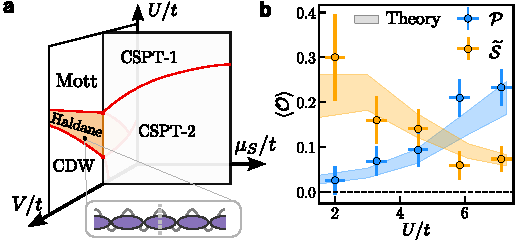
\includegraphics[width=247pt]{figures/Fig_Haldane_V3.pdf}
    \caption{\textbf{Haldane-Mott绝缘体相变。}偶极玻色- Hubbard模型中一个著名的SPT相是Haldane绝缘体(HI)相,该相可与CSPT-2相连通。\textbf{a},当交错场关闭时,在存在非局域相互作用($V$)的情况下,CSPT-1和-2相会转变为Mott绝缘体与Haldane绝缘体。插图中展示了由式~\eqref{eq:model-wavefunction}描述的HI相波函数示意图。\textbf{b},我们在固定$V/t\approx3$且无交错场$\mu_S$的条件下调节在位相互作用$U$。序参量的测量结果与模拟数据高度吻合。垂直误差棒通过自助法标准误差获得;水平误差棒为估计标准误差。}
    \label{fig: HI}
\end{figure}
\section{结论与展望}

我们的研究表明,当在晶体对称性保护拓扑(CSPT)相之间进行探测时,可以触及Haldane绝缘体(HI)与Mott绝缘体(MI)相变处的拓扑临界性。这凸显了可调量子模拟器的强大能力——它们能访问广阔的参数空间,并使得研究其他条件下难以企及的量子临界性成为可能。虽然局域观测量在远离原子极限时无法区分这些物相,但我们识别出了HI-MI相变和CSPT相变的非局域弦序参量。理论预测这两个相变都会呈现堆叠行为,这种行为定义了SPT的群结构并证实了其可逆特性。我们通过跨越CSPT临界点的动态扫描实验验证了这一性质。在CSPT体系中,我们还观测到混合态序的涌现,这将拓扑不变量推广到了混合态范畴。

我们在允许原子极限的一维物相间发现量子相变的现象,为更高维度中类似现象的研究开辟了可能性——这将成为理论与实验探索的新方向。这些相变可能有助于绘制拓扑平庸与非平庸相之间的绝热路径,从而激励人们从实验可制备的乘积态(如顺磁体~\cite{Scholl2021, Ebadi2021})出发,开发发现物态的新方法~\cite{Semeghini2021}。与此同时,我们对混合态序的演示引发出若干深刻问题:其稳定性如何?中间相的本质是什么?混合态视角如何深化我们对真实量子系统的理解?具体而言,该方法可用于实现依赖无序才能存在的平均晶体对称性拓扑相\cite{Ma23_b,intrinsicACSPT}。此外,比较通过显式对称性破缺与本文演示的堆叠性质来制备SPT相的保真度也颇具意义——后者对于制备受粒子宇称对称性等保护的二维SPT相可能特别有用\cite{LevinGu},因为这些对称性往往难以显式破坏。

研究结果强调,即使看似简单的模型也可能蕴含非平庸拓扑,这再次印证了拓扑工具不仅是抽象概念,更是识别和分类量子物相的实用框架。

\vspace{4pt}

\textbf{附注.} 在定稿期间,我们注意到关于数字量子器件中混合态序的预印本~\cite{Zhang2025},以及关于里德伯光镊量子模拟器中平均SPT的预印本~\cite{Yue2025},它们与本文预印本同期发表。
\section*{补充材料}


\subsection*{实验细节}


\subsubsection*{模型校准}

现场相互作用($U=U_\textrm{s}+U_\textrm{dd}$)通过调制晶格强度进行测量。我们装载单位填充的莫特绝缘体,调制晶格强度,保持与双激子寿命相当的时间,最后测量原子数。莫特绝缘体区域的共振频率$\nu$由$h\nu\approx U_\textrm{s}+U_\textrm{dd}-V_\textrm{nn}$给出~\cite{Chomaz2016}($V_{nn}$沿晶格调制方向)。我们计算了现场($U_\textrm{dd}$)和非现场($V$)偶极相互作用贡献,考虑了有限的Wannier(-Stark)函数。我们的模型与不同偶极角度和晶格深度的实验测量结果吻合良好。由于Wannier函数尺寸有限,非现场偶极相互作用($V$)并不严格遵循$1/r^3$衰减~\cite{Wall2013}。相反,前几个最近邻的相互作用大致按$1/r^{2.7}$衰减,这不会改变本文研究相的本质。隧穿能量($t$)通过强度调制测量晶格深度后计算得出。交错化学势($\mu_S$)通过强度调制校准。在没有手风琴晶格的情况下,固有(非可编程)化学势无序度估计为$\pm h\times$ 2.5~Hz,比哈密顿量中明确写出的最小能量尺度($t$)小近4倍,对于实现类Haldane绝缘体态足够小~\cite{Deng2013, Lv2018}。实现Haldane绝缘体时的超交换能量($t^2/U$)约为3~Hz,在实现CSPT时几乎可以忽略。密度诱导隧穿为-0.6~Hz~\cite{Baier2016},比隧穿能量小一个数量级以上,因此我们予以忽略。

\begin{figure}
    \centering
    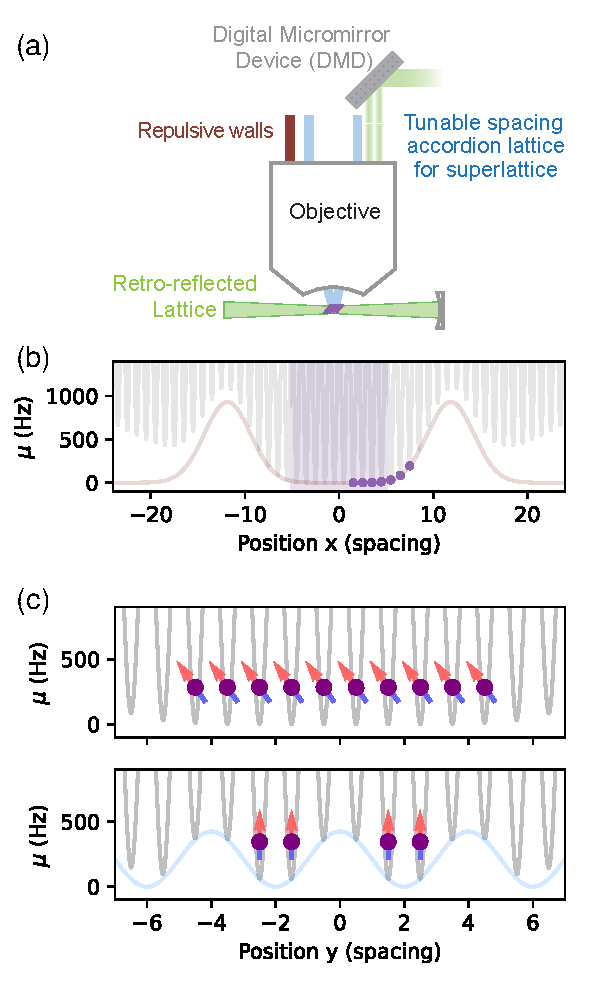
\includegraphics[width=0.48\textwidth]{figures/chemical_potential.pdf}
    \caption{\textbf{化学势。} \textbf{a},我们的显微镜可实现三种势场投影:利用蓝色手风琴晶格投影超晶格、通过数字微镜器件(DMD)投影任意势场、以及用蓝失谐椭圆光束投影相对尖锐的排斥势垒。\textbf{b},10位点系统沿一维链的化学势分布示意图。通过DMD补偿谐波约束与栗色标示的排斥势垒对后,中央紫色阴影区域的10个位点构成了定义明确的系统。紫色圆点标记的上升势垒遵循正文所述的化学势分布。\textbf{c},为提高数据采集速率,我们并行模拟多组链系统。上图通过提升晶格深度抑制链间隧穿,并倾斜磁场以最小化链间偶极-偶极相互作用;下图则利用浅蓝色超晶格构建隔离的双链体系。}
    \label{fig: chemical_potential}
\end{figure}
\subsubsection*{势场调控与边界条件}

如图~\ref{fig: chemical_potential}a所示,多种光学势场通过物镜进行投射。我们使用532纳米数字微镜器件(DMD)经物镜投射,以补偿红失谐光学晶格产生的谐波约束。此外,该装置还被用于引入可编程的化学势无序(图~\ref{fig: CSPT_average})。由于物镜存在定制通孔,我们的投射分辨率受到限制。无序图案通过叠加50个具有随机振幅、相位和空间频率的正弦波生成,这些参数均从均匀分布中采样:振幅范围0Hz至50Hz,频率范围0至1/(4个格点),相位范围0至$2\pi$。最终生成的无序图案具有有限关联长度,通过指数函数拟合$\langle\mu_i \mu_{i+d}\rangle$可量化为1.1个格点。其空间频率域谱类似于具有圆滑截止的白噪声。

为实现具有相对锐利边缘的有限长链,同时最小化系统中心区域引入的无序,我们通过物镜投射蓝失谐椭圆光束作为排斥势垒\cite{Gaunt2013}。该光束相对于841纳米处自然线宽为8千赫兹的跃迁约有400兆赫兹的失谐量。当交流斯塔克位移为数百赫兹时,我们估算其离共振散射率约为数十毫赫兹,与532纳米光学晶格的离共振散射率相当。进一步增加失谐量可改善离共振散射率,直至受限于激光器的放大自发辐射背景。边界条件在我们研究有限尺寸系统中类Haldane绝缘态时起着关键作用。数值模拟表明,边缘处化学势的平缓上升有助于增强Haldane弦序参量(公式~\eqref{eq: SOP})。如图~\ref{fig: chemical_potential}b中紫色圆点所示,边缘附近的化学势估计为[0,1,3,10,32,85,191]~Hz(对比参数$U\sim V=24$~Hz)。
\subsubsection*{实验步骤}

我们首先在2秒内制备出$^{164}$Er的玻色-爱因斯坦凝聚体(由于同位素丰度降低和散射长度减小,实验速度较~\cite{Phelps2020}有所减缓)。随后将该BEC压缩至一维垂直光晶格中,并通过排斥势垒进一步蒸发,直至目标区域达到所需原子数。接着以绝热方式将二维光晶格强度提升至目标隧穿强度$t$:初始采用80毫秒的指数型斜坡(时间常数$\tau = 40$毫秒),使晶格深度达到约三个反冲能量;随后通过线性斜坡调整晶格深度至目标隧穿强度(CSPT测量耗时120毫秒,MI-HI测量耗时200毫秒)。与此同时,通过物镜投射的超晶格线性提升交错化学势$\mu_S$,从而实现从BEC(超流体)到目标物相的转变。针对图3所示的CSPT-1相制备完成后,我们在100毫秒内线性调节$\mu_S$,同时以抛物线形式调节垂直晶格深度(产生$t_\perp$)。
\subsubsection*{并行数据采集}

为加速除图3外所有测量的数据采集过程,我们在每次实验中并行模拟约10条解耦的一维链(图~\ref{fig: chemical_potential}c顶部)。通过将晶格深度调节至链间隧穿强度比链内隧穿低一个数量级以上(链内隧穿本身已是哈密顿量(1)中的最小项),从而实现链间隔离。对于需要模拟两条耦合链的图3实验,我们引入额外超晶格在每对链之间插入两行空位(图~\ref{fig: chemical_potential}c底部)。这些空位行的化学势高出300~Hz,可抑制粒子泄漏并允许最高100~Hz的链间隧穿。每次实验并行运行2条耦合链。
\subsubsection*{单位填充哈伯德CSPT、半填充哈伯德CSPT与自旋1/2 XXZ CSPT的等价性}

\begin{figure*}
    \centering
    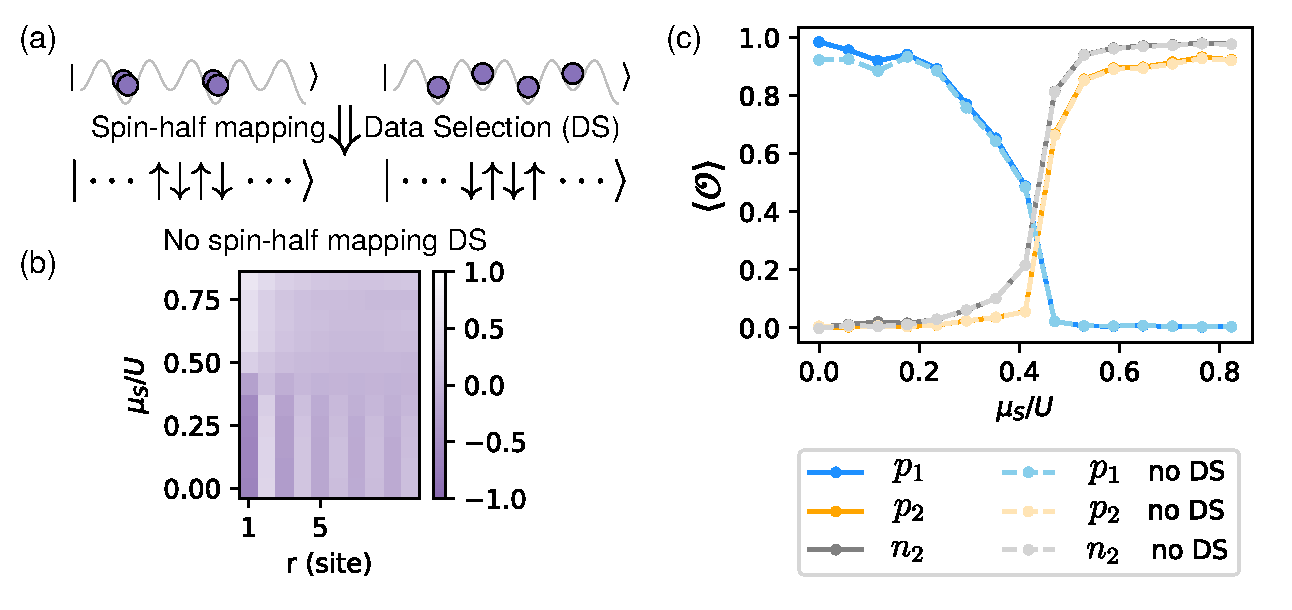
\includegraphics[width=\textwidth]{figures/DS.pdf}
    \caption{\textbf{自旋-1/2映射数据选择(DS).} \textbf{a}, 我们在正文中论证了自旋-1/2映射DS对于降低噪声的有效性。\textbf{b}, 我们展示了正文图2b中未应用自旋-1/2映射DS的数据。CSPTs的信号仍然存在——在底部区域我们观察到交错值,而在顶部区域我们观察到大致均匀的值。\textbf{c}, 在没有读出保真度等实验缺陷的模拟结果中,使用与不使用自旋-1/2映射DS计算的序参量在量子临界点附近相互重合。
    }
    \label{fig: spin_half_DS_extended_data}
\end{figure*}

在$t, V\ll U, \mu$的极限下,我们可以将具有交错化学势的单位填充哈伯德模型映射为一个有效自旋1/2 XXZ模型,其哈密顿量为

\begin{equation}
\label{eq: XXZ_Hamiltonian}
\begin{split}
H=-\frac{t}{\sqrt{2}}\sum_{\langle i,j \rangle}(X_iX_j+Y_iY_j)+\frac{V}{4}\sum_{\langle i,j \rangle}Z_iZ_j-\\\frac{1}{2}(\frac{U}{2}-\mu_S-V)\sum_i(-1)^iZ_i.
\end{split}
\end{equation}

通过映射到这个有效模型(图~\ref{fig: spin_half_DS_extended_data}a),我们可以执行数据选择(DS)来增强单位填充CSPT的信号。在具有吸引型交错势的格点上,数据选择标准为一个或两个玻色子;在具有排斥型交错势的格点上,选择标准为零个或一个玻色子。这种DS有效地减少了系统中双占据态到空态跃迁带来的噪声,帮助我们探测更大距离$r$处的$\mathcal{P}_{x_0}(r)$。为了证明自旋1/2映射是有效的DS判据,我们展示了两组额外数据。首先展示未应用该DS的实验数据,结果表明虽然由于实验缺陷导致测量噪声更大(图~\ref{fig: spin_half_DS_extended_data}b),但CSPT信号仍然存在。接着我们展示了不考虑任何实验缺陷的DMRG模拟结果(图~\ref{fig: spin_half_DS_extended_data}a)。可以看到在量子临界点附近,DS处理前后的结果没有显著差异。

该映射也可推广至半填充哈伯德模型,我们利用此模型研究耦合CSPT链,以增强有限尺寸下的能隙对比度。
\subsubsection*{数据筛选(DS)}

\begin{table*}[ht]
\begin{ruledtabular}
\begin{tabular}{p{0.04\linewidth} | p{0.09\linewidth} | p{0.1\linewidth} | p{0.09\linewidth} | p{0.08\linewidth} | p{0.12\linewidth} | p{0.08\linewidth} | p{0.09\linewidth} | p{0.09\linewidth} | p{0.09\linewidth}}
    Fig & System size (sites) & Atom number required & Atom number DS & Photon count DS & Spin-half mapping DS & Overall DS & Smallest sample size & Average sample size & Total sample size \\
    \hline
    2 & 16 by 1 & 16 & 9.0\% & 41.7\% & 36.2\% & 1.36\% & 197 & 660 & 7261 \\
    3 & 10 by 2 & 10 & 13.1\% & 86.8\% & Not needed & 11.4\% & 250 & 331 & 2975 \\
    4\textbf{a} & 10 by 1 & 10 & 8.1\% & 62.7\% & 53.3\% & 2.72\% & 74 & 204 & 1429 \\
    5 & 10 by 1 & 10 & 8.6\% & 47.4\% & Not applicable & 4.06\% & 99 & 130 & 649
\end{tabular}
\end{ruledtabular}
\caption{\label{tab:data_size} 我们应用两到三个步骤的数据筛选(DS)并展示DS率。基于系统中的总原子数进行DS,以减少初始态制备错误或斜坡与成像过程中损耗的影响。在满填充软核情况下,我们忽略每个格点含三个及以上粒子的链;在半填充硬核情况下,忽略每个格点含两个及以上粒子的链对。此外,基于每个格点的光子计数进行DS,当存在大量双粒子态或三粒子态或系统尺寸较大时,DS率较低。某些情况下还基于自旋1/2模型的映射进行DS。图3数据因映射至半填充交错偶极玻色-哈伯德模型,无需自旋1/2映射DS。图5数据在研究HI相时,由于不再投影交错化学势,自旋1/2映射不适用。表格展示了DS后的最终链数(图3中为双链数)。每次实验并行实现多条链(或双链),并对每条链独立进行DS。}
\end{table*}

在获取实验快照后,我们对原始光子计数进行处理并对每个格点的占据数进行数字化。当某格点的光子计数过于接近数字化阈值时,我们将该链(或多链)数据剔除。同时,我们统计链(或多链)中的总原子数,并舍弃不符合预期占据数的数据。在研究图~\ref{fig: Coupled_CSPT}中映射至半填充状态的隧穿耦合双链系统时,我们统计双链系统的总原子数,要求玻色子数目等于双链系统格点数的一半。特别地,在研究单位填充的CSPT时,我们通过将系统映射至自旋-1/2哈密顿量,额外施加一项数据筛选——剔除不属于自旋-1/2基的数据。数据筛选率及最终数据集规模详见表~\ref{tab:data_size}。需要强调的是,数据筛选仅用于增强信号特征,我们所研究的相态并非后选择的结果。
\subsubsection*{耦合链模拟的映射方法}

为了在原子数守恒的系统中对主文本公式~\eqref{eq: coupling}中的$H_\perp$耦合进行量子模拟,我们将单位填充的CSPT态映射至半填充态,并对底层实施粒子-空穴变换——将底层存在的\textit{物理玻色子}视为空穴(主文本图~\ref{fig: Coupled_CSPT}a底部)。在此表示下,配对项($\Delta_\perp$)转化为可实验实现的层间跃迁项($t_\perp$)。交错势场通过对角超晶格产生,最终形成棋盘格图案。
\subsubsection*{单点位点的二体与三体非弹性损失}

非弹性损失会降低基态保真度并损害量子模拟器的DS速率。我们注意到,当远离Feshbach共振时,非弹性损失率处于最佳状态~\cite{Chin2010, Frisch2014}。选用$^{164}$Er同位素是因为其有效S波散射长度可在远离Feshbach共振的低场区调节至所需值~\cite{Patscheider2022}。通过无宇称投影的位点分辨成像技术~\cite{Su2024},我们在主波长532纳米的晶格中测得双粒子态的寿命超过1秒,三粒子态寿命超过150毫秒。作为对比,我们典型的绝热演化时长为150毫秒,在绝热过程的大部分时段内双粒子和三粒子占据数并不显著。488纳米波长手风琴晶格的展开过程还需额外80毫秒,且实验测得双粒子寿命与Wannier函数尺寸高度相关。由于这些非理想因素,图2c中的观测量并未严格趋近于零。
\subsection*{数值模拟}


\subsubsection*{斜坡过程模拟}
\begin{figure}
    \centering
    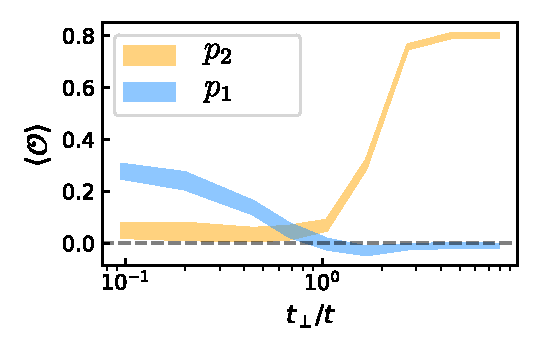
\includegraphics[width=0.48\textwidth]{figures/Coupled_CSPT_OP_gnd_state_no_decoherence.pdf}
    \caption{\textbf{无任何退相干情况下的模拟序参数。} 正文图3展示了考虑对角超晶格导致的退相干效应后模拟的序参数。此处我们呈现无任何退相干时的模拟结果,可以观察到序参数存在相对尖锐的交叉转变。
    }
    \label{fig: Coupled_CSPT_no_decoherence}
\end{figure}

\paragraph*{CSPT模拟} 图中阴影部分的理论计算是通过ITensor环境中的张量网络算法~\cite{itensor},在有限尺寸系统中模拟从超流体到最终态的斜坡过程实现的。基态计算采用密度矩阵重整化群(DMRG)方法,设置最大键维数$\chi_m=300$和矩阵乘积态(MPS)压缩的截断误差阈值$\epsilon \approx 10^{-12}$。实验中的精确斜坡序列通过Trotter分解和含时演化块消减(TEBD)实现,其中每步设置$\chi_m=300$、$\epsilon \approx 10^{-10}$及时间步长$dt=0.2$ms。所有模拟设定每个格点的最大玻色子数为3。我们还考虑了实验中存在的粒子数涨落,即链长$L$附近$N=L, L\pm1, L\pm2$粒子的构型。这些涨落对模拟实验条件至关重要,研究发现即使在基于总粒子数的数据筛选(DS)后,由于损耗和成像误差等因素,粒子数涨落仍会轻微抑制整个相图中的CSPT序参量。对于HI-MI相变的模拟,我们考虑了高斯型势阱壁的边界条件。

图~\ref{fig: Coupled_CSPT}所示实验采用对角超晶格来投影所需棋盘格图案的化学势。实验观察到,相较于使用非对角超晶格的其他实验,该化学势激光会引起显著加热效应。这种加热导致实验中不可忽略的退相干,必须建模才能准确反映实验结果。若不考虑退相干,模拟结果如图~\ref{fig: Coupled_CSPT_no_decoherence}所示。我们选择用经典白噪声模拟耗散时间演化,以此模拟具有跳跃算符$\hat n_i$的Lindblad主方程~\cite{Kampen1992, Seif2022}。为忠实反映具有关联经典白噪声的耗散动力学,我们在哈密顿量(式~\eqref{eq: Hamiltonian})中引入时变化学势$H_{\rm wn}=\sum_i \mu_i(t) \hat  n_i$。其中$\mu_i(t)$服从$\braket{\mu_i(t)}=0$和$\braket{\mu_i(t)\mu_j(t')}=\gamma_{ij}(t) \delta(t-t')$的正态分布,协方差矩阵$\Gamma(t)=\left[\gamma_{ij}(t)\right]=\sigma(t)\mathcal{I}$表示$t$时刻的经典白噪声,即不同格点$i$的$\mu_i(t)$采样自均值为0、标准差为$\sigma(t)$的高斯分布。由于对角超晶格同时调控交错势$\mu_s(t)$,我们将$\sigma(t)$与$\mu_s(t)$关联调制:$\sigma(t)=\sigma_0 |\mu_s(t)|/\textrm{max}(|\mu_s(t)|)$。这意味着在CSPT深区(如$\mu_s \approx \pm 100$~Hz)退相干最强,而在临界点附近(如$\mu_s=0$)可忽略。通过该模型,发现$\sigma_0=20$~Hz能准确复现图~\ref{fig: Coupled_CSPT}b中所有$t_\perp/t$的实验结果。

需特别说明,虽然退相干效应不可忽略,但通过将实验数据与小尺寸系统的精确对角化(ED)结果对比,我们估算体系温度仍低于能隙的一半,这使得我们能够有效探测基态物理。

\paragraph*{MI-HI模拟} 为模拟从MI到HI的斜坡过程,我们采用前一节描述的边缘化学势对16个格点进行模拟。数值计算使用Tensor Network Python(TeNPy)~\cite{Hauschild18}完成。研究发现对于所考虑的系统参数,最大键维数$\chi_{\text{max}} = 182$足以保证收敛性。模拟过程首先通过DMRG寻找不同总原子数超流体的基态作为初态,随后采用文献~\cite{Zaletel2015}发展的基于矩阵乘积算符的方法进行动力学斜坡模拟,设置Trotter步长$dt = 0.1 \text{ ms}$。
\subsubsection*{基态模拟}

\paragraph*{局域观测量在大系统尺寸下仍保持非锐化特性}

\begin{figure}
    \centering
    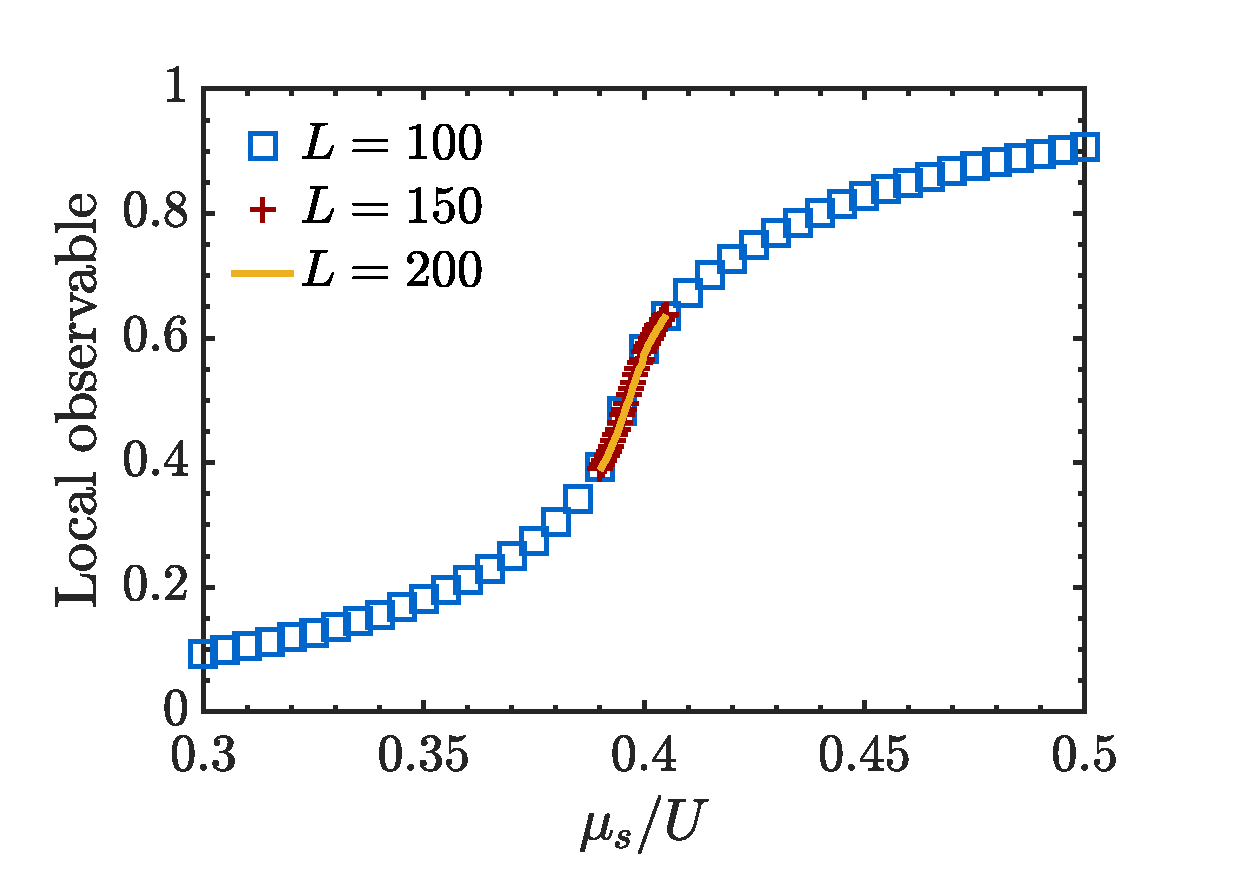
\includegraphics[width=0.48\textwidth]{figures/large_size_local_observable.pdf}
    \caption{\textbf{更大系统尺寸的数值模拟表明局域观测量仍保持非锐化特性。} 为证明图2中局域观测量的非锐化现象并非源于有限系统尺寸,我们通过DMRG模拟研究了更大尺寸体系并绘制了$n_2$的变化曲线。参数设置:U/t=20,V/t=2.5,每个格点的原子数截断为4,偶极相互作用尾部根据实验值保留。}
    \label{fig: large_size_local_observable}
\end{figure}

正文图2中,我们展示了局域观测量$n_2$的平滑变化特性,并指出其不能作为序参数使用,因为在CSPT-2相外该量不为零。我们的实验系统尺寸为有限值$L=16$个格点。为论证该行为并非源于有限尺寸效应,我们采用DMRG方法模拟了$L=100, 150$及$200$格点的系统,观测到相同的平滑特性,如图~\ref{fig: large_size_local_observable}所示。

\paragraph*{多重$\mathbb{Z}_2$ CSPT的耦合效应}

\begin{figure}
    \centering
    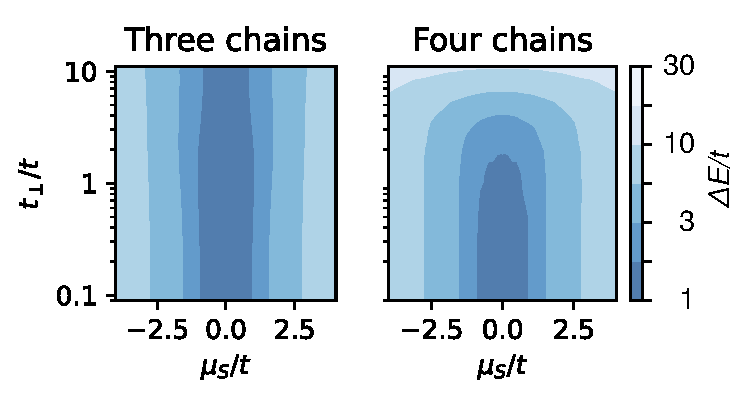
\includegraphics[width=0.48\textwidth]{figures/three_or_more_coupled_chains.pdf}
    \caption{\textbf{耦合多条 CSPT 链的能隙模拟。} 耦合三条(奇数条)链会重新激发两相之间的量子相变,这可以通过平行的等高线观察到。耦合四条(偶数条)链产生的能隙与耦合两条链的情况类似,在高 $t_\perp$ 值下能隙闭合现象消失。
    }
    \label{fig: three_or_more_coupled_chains}
\end{figure}

正文中我们指出解耦链具有两种拓扑不同的CSPT态,但两条隧穿耦合链会使拓扑性平庸化。通过精确对角化(ED)方法(\textsc{QuSpin}~\cite{QuSpin})对3×8格点和4×6格点系统进行数值模拟,我们进一步研究了更多耦合链情况下的$\mathbb{Z}_2$特性,结果如图~\ref{fig: three_or_more_coupled_chains}所示。

\paragraph*{CSPT与MI-HI量子相变间的插值研究}

\begin{figure*}
    \centering
    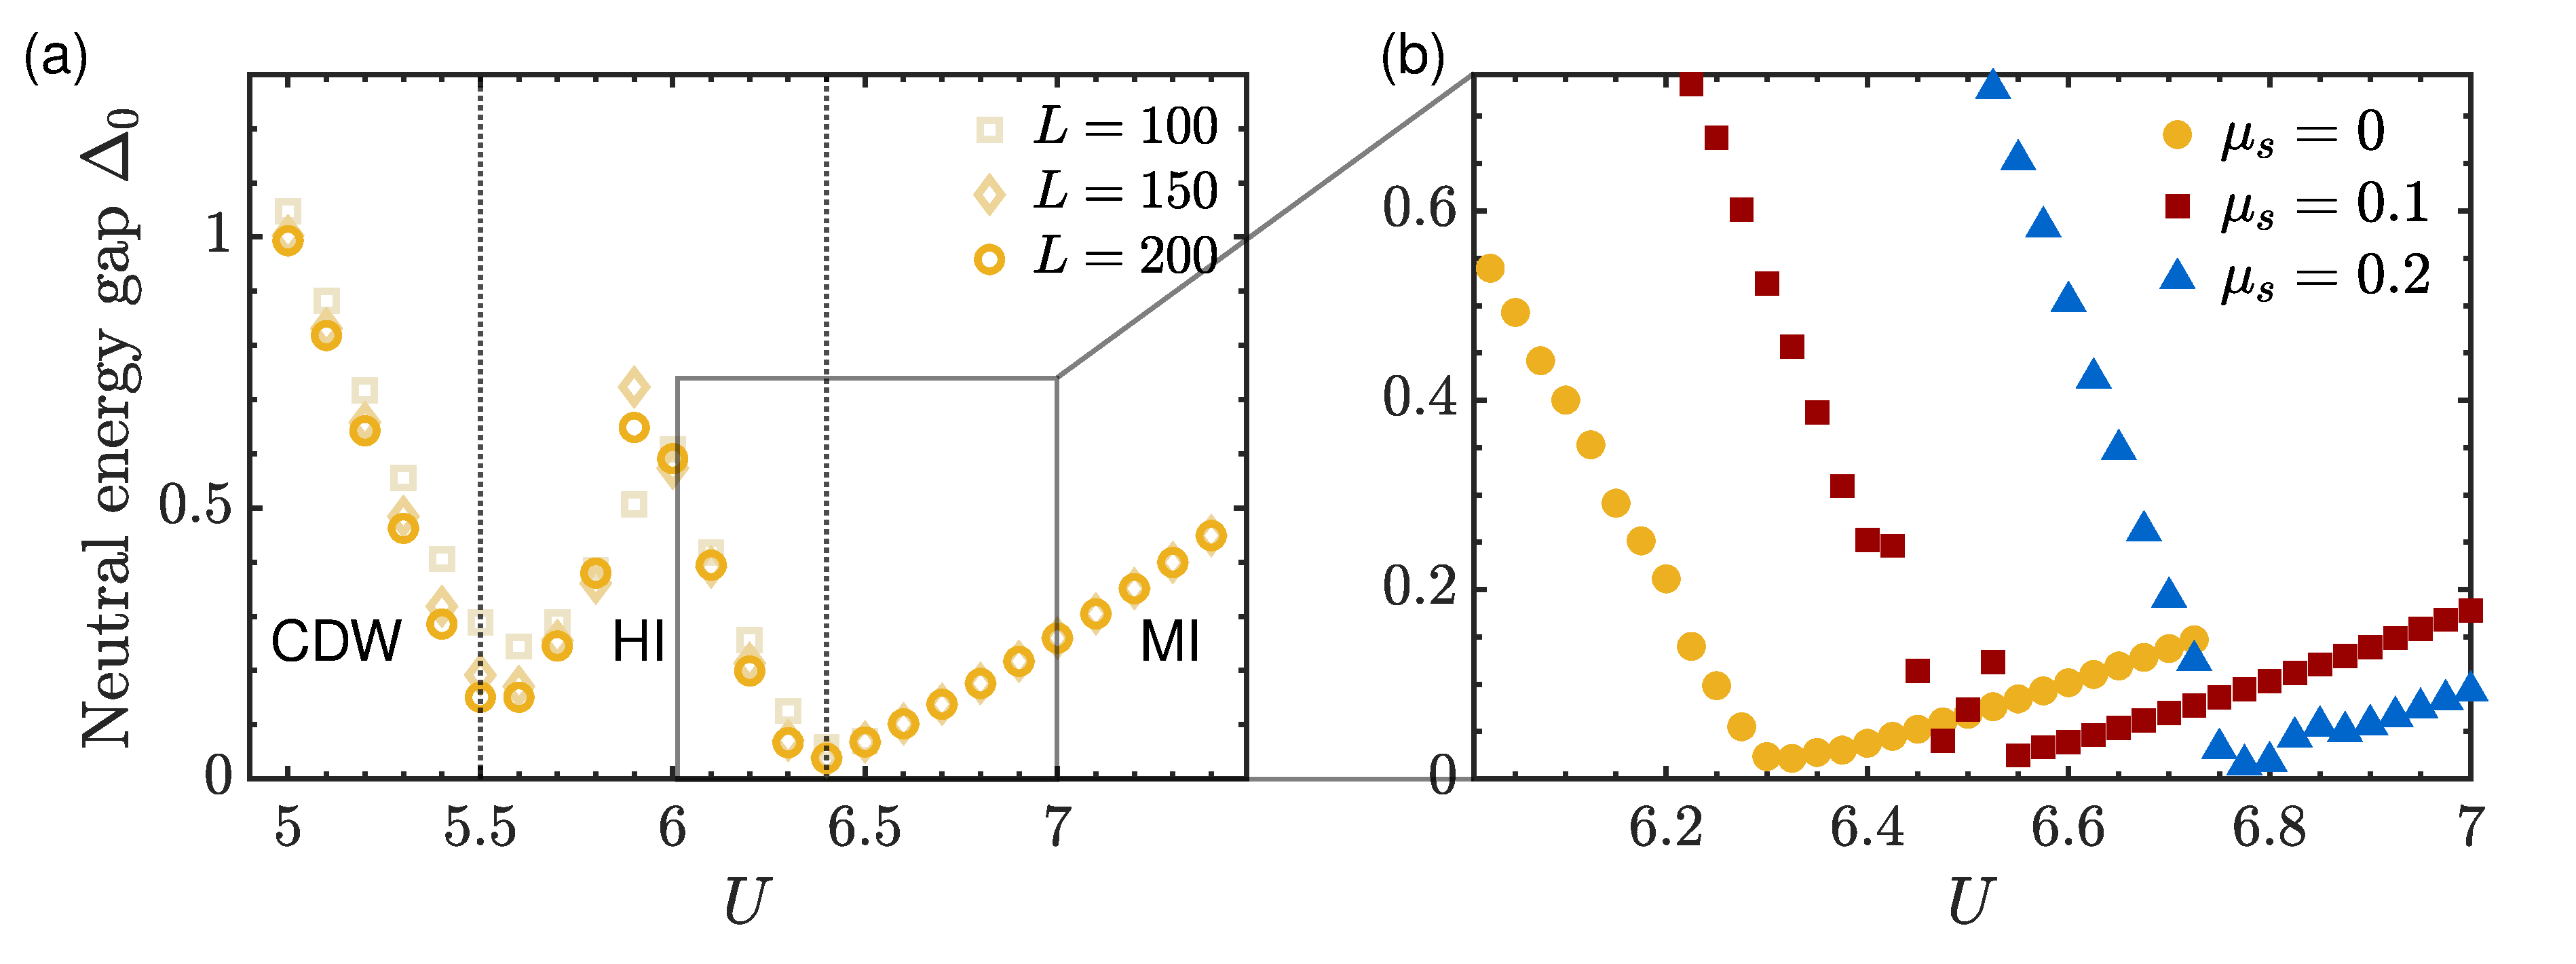
\includegraphics[width=\textwidth]{figures/HI_to_CSPT_transition_large_size.pdf}
    \caption{\textbf{模拟能隙揭示了MI-HI相变与CSPT相变之间的关联。} \textbf{a},不同系统尺寸 ($L$) 下 $\mu_S=0$ 处MI-HI相变的能隙。\textbf{b},在固定系统尺寸 $L=256$ 格点时开启 $\mu_S$,MI-HI相变会过渡至CSPT相变。本图中所有模拟均采用最近邻相互作用且每格点最大玻色子数为2,以确保DMRG计算的快速收敛。
    }
    \label{fig: HI_to_CSPT_transition_large_size}
\end{figure*}

图~\ref{fig: HI_to_CSPT_transition_large_size}展示了中性激发的能隙$\Delta_0=E_1-E_0$,其中$E_0$和$E_1$分别表示单位填充条件下固定系统尺寸的基态与第一激发态。子图a呈现了CDW、HI和MI相之间两个相变点的能隙闭合现象,该特征随系统尺寸增大而愈发显著。子图b聚焦HI-MI相变,展示了引入交错化学势$\mu_s$后MI-HI相变如何转变为CSPT相变。
\subsection*{理论分析}

本节我们将为实验结果的背后理论分析提供更多细节说明。尽管以下内容已使当前研究工作自成体系,但更全面且具有教学意义的理论阐述将在即将发表的文献\cite{Sahay2025}中予以呈现。
\subsubsection*{晶体对称性}
我们首先对有限系统的晶体对称性本质作简要说明。严格来说,仅当系统长度为奇数时,才具有以格点为中心的反演对称性。然而,对于物质的体相性质而言,这种系统尺寸奇偶性的区别不应产生影响。
\subsubsection*{CSPT拓扑不变量}

为了直观理解区分CSPT-1和CSPT-2的拓扑不变量,我们首先考察原子极限下出现的乘积态。区分这两种态的一种方法是:在任何大范围反演对称区域内,CSPT-1和CSPT-2中玻色子的宇称分别为$-1$(奇)和$+1$(偶)(主文本图~\ref{fig: CSPT_ground}a中CSPT-1的上半部分)。当引入量子涨落并远离原子极限时,这些态中的玻色子会退局域化为修饰准粒子(主文本图~\ref{fig: CSPT_ground}a下半部分),此时该区域内宇称的期望值不再严格等于$+1$或$-1$。然而,这些区域内宇称期望值的\textit{符号}仍可作为区分两者的离散不变量。

只要能隙保持开放且宇称与反演对称性均未被破坏,该区域内宇称期望值的任何变化都会从其边缘对称地发生。因此,体宇称的符号始终保持不变(主文本图~\ref{fig: CSPT_ground}a下半部分)。推导该不变量所需的技术工具见文献~\cite{Fuji2015},其推导过程与后文补充材料中混合态不变量的推导密切相关。
\subsubsection*{SPT相中局域序参量的缺失}
朗道范式通过表征自发对称性破缺的局域序参量来刻画相变~\cite{Landau1937, Beekman2019}。与之形成鲜明对比的是,我们研究的相变位于该框架之外:它分隔了两个无法通过任何局域观测量区分的对称保护拓扑(SPT)相。虽然诸如平均格点占据数等局域观测量会对交错化学势产生响应,但它们无法作为区分这两种晶体SPT相的序参量。这是因为哈密顿量已经显式地破坏了平移对称性,因此即使在平庸相中,密度调制也始终存在——并且它们在相变过程中平滑变化。要成为序参量,观测量必须在相外为零而在相内非零。相比之下,区分这两个相位的拓扑不变量(例如,空间反演对称性宇称弦的符号)会发生突变,并且受到对称性和有限能隙的保护~\cite{Fuji2015, Pollmann2012}。

更形式化地说,我们注意到任何两个对称的、短程纠缠基态都无法通过局域观测量的期望值来区分,因为对称的、有限深度的局域幺正电路可以将局域算符映射到其他局域算符,而不改变对称性约束~\cite{Chen2010, Chen2011}。因此,任何对称局域观测量的期望值总能在不同SPT相之间平滑形变,因而无法作为尖锐的序参量。
\subsubsection*{混合态有序性的理论框架}
混合态有序性的实验实现可形式化表述如下:我们从分布$p_{\mathcal{D}}$中抽取无序构型$\mathcal{D}$,使得通过格点中心反演相关联的无序模式具有相同概率。对于每个无序构型,其基态$\ket{\psi_{\mathcal{D}}}$可通过以下方式探测:
\begin{equation}
    \mathbb{E}[\mathcal{P}_{x_0}(r)] = \sum_{\mathcal{D}} p_{\mathcal{D}} \bra{\psi_{\mathcal{D}}} \hat{\mathcal{P}}_{x_0}(r)\ket{\psi_{\mathcal{D}}}.
\end{equation}
关键的是,上述探测等价于实验测量混合态$\rho = \sum_{\mathcal{D}} p_{\mathcal{D}} \ket{\psi_{\mathcal{D}}} \bra{\psi_{\mathcal{D}}}$中宇称弦算符的期望值$\mathbb{E}[\mathcal{P}_{x_0}(r)] = \text{Tr}\left( \rho\,  \hat{\mathcal{P}}_{x_0}(r)\right)$。我们将证明,只要链的格点中心反演对称性在平均意义上得以保持,所研究的晶体对称性保护拓扑(SPT)相就会持续存在。

在深入证明之前,我们先回顾混合态多体物理中的若干基础概念:
\textit{混合态中的短程纠缠与对称性}。将SPT概念从纯态推广至混合态时,必须同时理解混合态的纠缠结构及其对称性。纯态SPT的核心特性在于其短程纠缠(SRE)性质——即可以通过局域哈密顿量的有限时间演化从乘积态制备得到。为讨论混合态SPT,我们需要建立适当的混合态推广方案。尽管文献中已出现多种定义\cite{Ma2023, Chen2024},本文采用如下表述:若混合态密度矩阵$\rho$定义在希尔伯特空间$\mathcal{H}_A$上,当存在SRE纯态$\ket{\psi_{\text{AB}}} \in \mathcal{H}_A \otimes \mathcal{H}_B$使得$\rho = \text{Tr}_{B}(\ket{\psi_{\text{AB}}} \bra{\psi_{\text{AB}}})$时,称$\rho$具有SRE性质。换言之,$\rho$若存在SRE纯化即视为SRE态。

定义了混合态SRE概念后,我们转向理解其对称性。对于混合态,对称性在概念上可分为两类:假设混合态$\rho_A$源于更大系统$\mathcal{H}_{A} \otimes \mathcal{H}_{B}$中的纯态,则该系统的对称性可能仅作用于$\mathcal{H}_A$或共同作用于$\mathcal{H}_A \otimes \mathcal{H}_B$。等效地说,守恒量可能仅存在于$A$子系统或在$A$与$B$间交换。第一种情况对应\textit{强对称性}(或称精确对称性),其由算符$U_A \otimes \mathds{1}_{B}$生成,混合态在$U_A$左乘或右乘下保持不变,即$U_A \rho_A = e^{i \theta} \rho_A$。第二种\textit{弱对称性}(或称平均对称性)则由算符$U_A \otimes U_B$生成,密度矩阵仅满足共轭不变性$\rho = U_A \rho U_A^{\dagger}$。

\textit{无序交错偶极玻色-哈伯德模型的SRE与对称纯化}。现在我们将证明,弱无序作用下交错偶极玻色-哈伯德(SDBH)模型基态系综是具有强$\mathbb{Z}_2$宇称对称性与平均格点中心反演对称性的SRE混合态。为此,我们显式构造该无序模型基态系综的SRE纯化态,该纯化需同时满足宇称对称性与反演对称性。假设各格点无序分布互不关联\footnote{此假设仅为简化讨论,实验中由于势场投影的有限分辨率并非严格成立},则化学势无序构型$\mathcal{D} = \{\mu_x\}$的概率为$p(\mathcal{D}) = \prod_{x} p_x(\mu_x)$。纯化构造如下:

设$H_A$为无无序的SDHB模型(式\eqref{eq: Hamiltonian}),处于$U$较大且$\mu_{\text{S}}$远离临界点的参数区。令$\mathcal{H}_B$为各格点定义实数值态$\ket{\mu_x \in \mathbb{R}}$的希尔伯特空间,满足$\langle \mu_x|\mu'_x\rangle =  \delta(\mu_x - \mu'_x)$,其哈密顿量为:
\begin{equation}
    H_{B} = -\Delta \sum_{x} \ket{p_x} \bra{p_x} \qquad \ket{p_x} = \int d\mu_x \sqrt{p_x(\mu_x)} \ket{\mu_x}
\end{equation}
其中$\Delta$将取无穷大极限。最后设定$A$与$B$系统间的耦合:
\begin{equation}
    H_{\text{AB}} = - \sum_{x} n_x \hat{\mu}_x
\end{equation}
其中$\hat{\mu}_x \ket{\mu_x} = \mu_x \ket{\mu_x}$。哈密顿量$H = H_{\text{A}} + H_{\text{B}} + H_{\text{AB}}$的基态(在$\Delta \to \infty$极限下)可用无序SDBH模型的基态表示。特别地,$H_B$将$\mu$自由度投影至$\ket{p_x}$态,而$H_{\text{AB}}$项使$A$系统感受到$B$系统的等效化学势。因此有:
\begin{equation}
    \ket{\psi_{\text{AB}}} = \sum_{\{\mu_x\}} \underbrace{\left(\prod_{x} \sqrt{p(\mu_x)} \right)}_{p_{\mathcal{D}}} \ket{\psi[\{\mu_x\}]}_{\text{A}} \otimes \ket{\{\mu_x\}}_{\text{B}}
\end{equation}
其中$\ket{\{\mu_x\}} = \bigotimes_x\ket{\mu_x}$,$\ket{\psi[\{\mu_x\}]}$为对应无序构型$\{\mu_x\}$的SDBH模型基态。注意到$\ket{\psi_{\text{AB}}}$正是SDBH模型基态系综的纯化:
\begin{equation}
    \rho_A = \sum_{\mathcal{D}} p_{\mathcal{D}} \ket{\psi_{\mathcal{D}}} = \text{Tr}_B\left(\ket{\psi_{\text{AB}}}\bra{\psi_{\text{AB}}}\right).
\end{equation}

此处需作几点说明:首先,哈密顿量$H$具有能隙——这是因为$H_B$严格可解且具有能隙,$H_A$本身有能隙,且在无序足够弱时$H_{\text{AB}}$作为微扰不会关闭能隙。因此$\ket{\psi_{\text{AB}}}$作为哈密顿量的唯一有能隙基态,可通过准绝热演化从乘积态制备而得,故具有SRE性质。由此,$\rho$确实允许SRE纯化。
此外注意到,由于$\ket{\psi_{\text{AB}}}$在$A$子系统的宇称变换下对称且满足$\mathcal{I}_A \otimes \mathcal{I}_B$的位点中心反演对称性,$\rho$具有强$\mathbb{Z}_2$宇称对称性以及所需的平均$\mathcal{I}_A$对称性。

\begin{figure*}
    \centering
    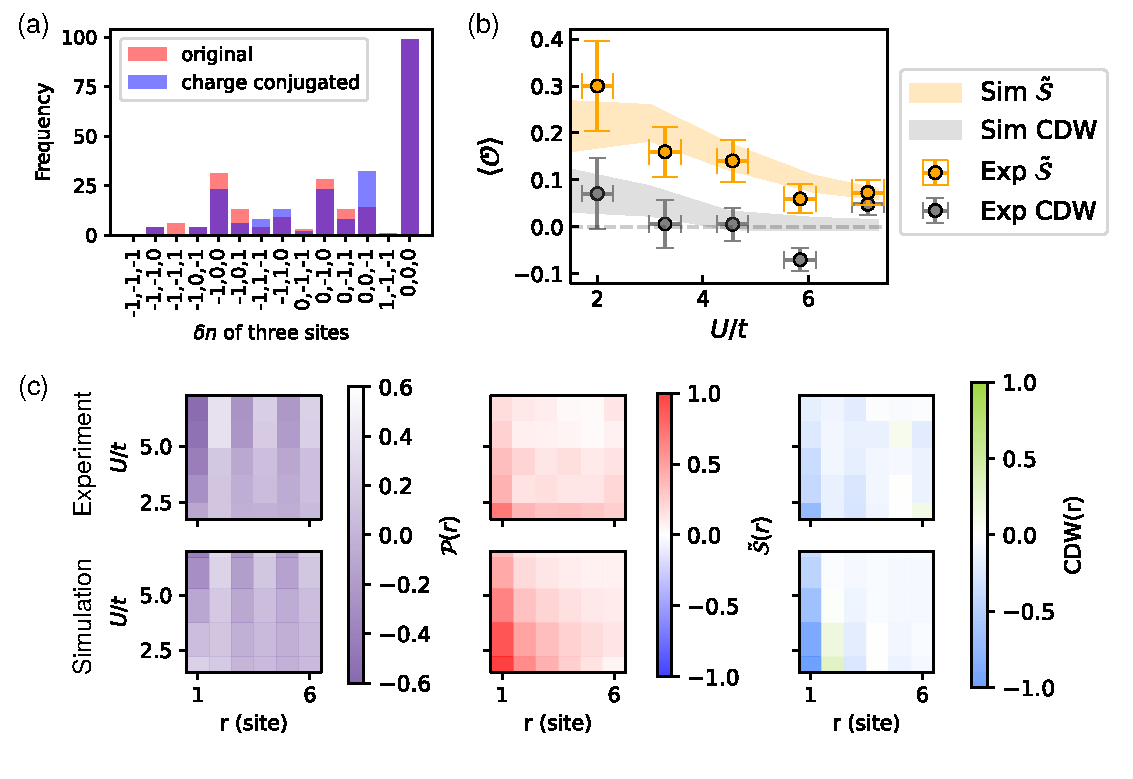
\includegraphics[width=\textwidth]{figures/HI_2D_OP.pdf}
    \caption{\textbf{莫特绝缘体到Haldane绝缘体量子相变的序参数。} \textbf{a},我们在系统中随机选取三个位点并绘制观测状态的直方图。原始(红色)与电荷共轭(蓝色)计数的相似性可作为近似电荷共轭对称性的实验证据。\textbf{b},通过比较归一化后的Haldane弦序参数与电荷密度波序参数,证明系统处于Haldane绝缘体区域。垂直误差棒通过自助法标准误差获得;水平误差棒为估计标准误差。\textbf{c},观测量相对于$r$的变化曲线。
    }
    \label{fig: HI_2D_OP}
\end{figure*}
\textit{精确宇称与平均反演对称性导出的平均SPT不变量。} 我们现在证明,宇称弦序参量测量了该系综中无法通过有限深度量子信道改变的拓扑不变量。
为此,假设$\rho$是一个强$\mathbb{Z}_2$对称性$\mathcal{P}_A$和弱位点中心反演对称性$\mathcal{I}_A$下的SRE混合态。
那么,$\rho$存在一个在$\mathcal{P}_A \otimes \mathds{1}$和$\mathcal{I}_A \otimes \mathcal{I}_B$下对称的SRE纯化态$\ket{\psi_{\text{AB}}}$。
因此,对于相距远大于关联长度$\xi$的$a, b$两点,$\mathbb{Z}_2$对称性弦算符$\mathcal{P}_{a, b}$在该态上分数化表现为:
\begin{equation}
    \mathcal{P}_{a, b} \otimes \mathds{1} \ket{\psi_{\text{AB}}} = q^L_a q^R_b \ket{\psi_{\text{AB}}}
\end{equation}
其中$q^L_a$和$q^R_b$分别是局域于$a$和$b$端点的酉算子(但可能同时作用于$A$和$B$子系统)。
需注意$q^L_a$和$q^R_b$的定义存在歧义:我们可以取$q_{a}^L \to e^{i \alpha} q_a^{L}$和$q_{b}^{R} \to e^{-i \alpha} q_a^{L}$而不改变上述关系(其中$\alpha \in U(1)$是与$a, b$无关的相位)。
通过要求$q_a^L$和$q_b^R$平方等于一(即形成$\mathbb{Z}_2$的表示),我们可以将这种自由度固定至符号差异,这之所以可行是因为$\mathcal{P}_{a, b}$平方等于一。
基于此,设$[a, b]$为链的奇数长度反演对称区域;不失一般性,可取$b = -a$。
在原点处的反演对称性$\mathcal{I}_0 = \mathcal{I}_{A, 0} \otimes \mathcal{I}_{B, 0}$作用下,我们有:
\begin{align}
    \mathcal{I}_{0} \mathcal{P}_{a, -a} \otimes \mathds{1} \ket{\psi_{\text{AB}}} &= (\mathcal{I}_0 q_{a}^L \mathcal{I}_0)(\mathcal{I}_0 q_{-a}^R \mathcal{I}_0) \ket{\psi_{\text{AB}}} \nonumber\\
    &= q_{a}^L q_{-a}^{R}\ket{\psi_{\text{AB}}} = \mathcal{P}_{a,-a} \ket{\psi_{\text{AB}}}
\end{align}
由此可得:
\begin{equation}
     (\mathcal{I}_0 q_{a}^L \mathcal{I}_0) = e^{i \Theta_a} q_{-a}^{R} \qquad (\mathcal{I}_0 q_{-a}^R \mathcal{I}_0) = e^{-i \Theta_a} q_{a}^{L}
\end{equation}
由于$q_a^{L/R}$平方等于单位算符,由上式可知$\Theta_a$只能取值$0, \pi$。
由于$\Theta_a$是表征该态的离散数,它无法通过$\rho$上的对称量子信道(等价于$\ket{\psi_{\text{AB}}}$上的FDLU操作)连续改变。
我们指出$\Theta_a$可通过下式提取:
\begin{align}
    \text{Tr}\left(\rho \mathcal{P}_{a, -a} \right) = \langle q_a^L q_{-a}^R \rangle_{\psi_{\text{AB}}} &\approx \langle q^L_a \rangle_{\psi_{\text{AB}}} \langle q^R_{-a} \rangle_{\psi_{\text{AB}}}\\
    &= e^{i \Theta_a} \langle q_a^L \rangle^2_{\psi_{\text{AB}}}
\end{align}
其中第二步源于SRE态的关联簇性质,最后一步利用了$\langle q_{-a}^R \rangle_{\psi_{\text{AB}}} = \langle \mathcal{I}_0 q_{-a}^R \mathcal{I}_0 \rangle_{\psi_{\text{AB}}} = e^{i \Theta_a} \langle q_a^{L} \rangle_{\psi_{\text{AB}}}$这一事实。
因此,奇数长度区域的宇称弦符号是表征该态的拓扑不变量。
需注意,原则上每一对反演对称的位点都存在一个拓扑不变量$\Theta_a$。
然而,在存在平移对称性的情况下(例如当位点中心反演对任意位点均为对称性时出现的双位点平移),仅有两个不变量保持独立\cite{Sahay2025}。
\subsection*{Haldane相到Mott绝缘体的相变}

在本补充材料章节中,我们将进一步阐释Haldane相与Mott绝缘体相变之间的关联,以及CSPT-1与CSPT-2相变之间的联系。

\begin{figure}
    \centering
    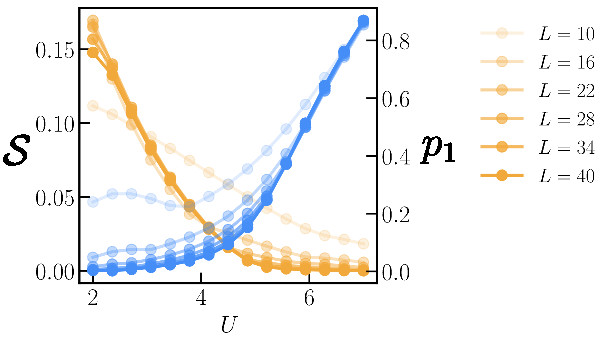
\includegraphics[width=0.48\textwidth]{figures/Finite_size_scaling.pdf}
    \caption{\textbf{MI-HI 相变的有限尺寸标度模拟。} 在较大系统尺寸下,序参量变化更为陡峭,表明存在量子相变。$V_\mathrm{nn}/t=3$,$V$ 遵循实验观测的 $1/r^{2.7}$ 衰减规律。每个格点的玻色子数截断至三个。}
    \label{fig: finite_size_scaling}
\end{figure}
\subsubsection*{MI-HI相变与CSPT相变之间的联系}

首先需要回顾的是,在不存在交错势($\mu_{\text{S}} = 0$)的情况下,理论预测偶极玻色-哈伯德模型的相图会随着在位相互作用强度$U$和长程相互作用特征强度$V$的变化而包含至少三个绝缘相(示意图见正文图~\ref{fig: HI}a)~\cite{Torre2006, Berg2008}。其中两个分别是莫特绝缘体(MI)和电荷密度波(CDW),后者在$\mu_{\text{S}} = 0$时自发地将模型的平移对称性$\mathbb{Z}$破缺至$2\mathbb{Z}$。最后一个相是霍尔丹绝缘体(HI)——这是一种处于$\mu_{\text{S}} = 0$时具有晶体\textit{键中心}反演对称性和宇称对称性的偶极玻色-哈伯德模型中的纠缠SPT相,它与莫特绝缘体之间通过量子相变分离~\cite{Pollmann2010}。从这个意义上说,HI是一种具有受保护量子纠缠的CSPT相。

为了理解霍尔丹-莫特绝缘体相变如何与CSPT-1和CSPT-2之间的相变相关联\cite{Sahay2025},我们注意到在加入交错势后,莫特绝缘体会明显地演化为CSPT-1相。为了直观理解HI与CSPT-2之间的关系,我们采用正文(第~\ref{sec:CSPT-transitions}节)中介绍的CSPT"修饰准粒子"图像。

具体而言,HI可以看作是我们系统中每个玻色子在晶格键上离域的情况,如正文图~\ref{fig: HI}a所示——这种构型保持了模型的宇称、格点中心与键中心反演对称性。该相的模型波函数具体表示为:
\begin{equation} \label{eq:model-wavefunction}
    \ket{\psi} \propto \bigotimes_{x} \left( b_{x}^{\dagger} + b_{x + 1}^{\dagger} \right) \ket{0},
\end{equation}
该表达式捕捉了键离域的特征。正文方程~\eqref{eq: SOP}中的弦序参量与我们用于CSPT-1和CSPT-2的宇称弦算符类似,但此时存在端点修饰项$\delta \hat n = \hat n-1$。这是因为若无此修饰,由于键离域玻色子在感兴趣区域内外的概率均等,预期宇称值将为零。修饰项的引入修正了这一效应,$\mathcal{S}_{x_0} (r)$的非零值(对于奇数长度)被预测为正,这与CSPT-2的现象学完全一致,揭示了两者的关联。需注意端点算符$\delta n$在链的近似电荷共轭对称性下会变换为$-\delta n$——正是这种端点修饰的变换规律成为了HI的拓扑不变量\cite{Pollmann2012, Schuch2011, Chen2011}。
\subsubsection*{近似电荷共轭对称性}
为了证明近似的电荷共轭对称性,我们分析了系统的中心3个位点并绘制了分布直方图。该分布相对于电荷共轭中心大致对称,从而验证了这一近似对称性。

这一分析为使用弦序参量$\mathcal{S}$识别HI态提供了理论依据,并进一步解释了有效弦观测量$p_1$($p_2$)在CSPT-$2$(CSPT-$1$)中消失的原因。
\subsubsection*{扩展数据}
我们在图~\ref{fig: HI_2D_OP}中展示了有限尺寸实验系统中从莫特绝缘体到Haldane绝缘体量子相变的可观测量二维彩色图。为区分Haldane绝缘体相与邻近的电荷密度波相,我们还绘制了归一化的两点密度-密度关联函数$\mathrm{CDW}(r)=\eta\langle \delta n_i \delta n_{i+r} \rangle$。通过主文中定义的$\eta$对两者进行归一化后,我们将CDW序参数与Haldane弦序参数进行了对比。

实验中可实现的有限尺寸(10个格点)限制了Haldane绝缘体与莫特绝缘体之间量子相变~\cite{Fraxanet2022}的锐度。为数值验证莫特绝缘体与Haldane绝缘体间的量子相变,我们采用密度矩阵重整化群(DMRG)进行了有限尺寸标度分析(图~\ref{fig: finite_size_scaling})。需要指出的是,我们的系统尺寸小于使用iDMRG方法在热力学极限下模拟得到的关联长度。实验系统中的无序和退相干效应可能会减小关联长度,但仍需强调本实验所探测的态可能处于量子临界区域,严格来说并非绝缘态。此外,限定系统尺寸的势垒墙并非无限陡峭,当$U$较大时可能出现原子向定义系统外部的泄漏。

未来量子气体显微镜技术的进步或可实现足够大系统尺寸下纠缠谱的测量,从而揭示偶极玻色-哈伯德模型中Haldane绝缘体相边缘模的特征~\cite{Deng2011, Tran2023}。
\section*{补充信息}

\paragraph*{数据与代码可用性}
支持本研究结果的实验数据与分析代码可根据合理请求向通讯作者获取。

\paragraph*{致谢}
实验团队感谢A. Hebert、A. Krahn、G. Phelps、R. Groth、S. F. Ozturk、S. Ebadi、S. Dickerson、F. Ferlaino、V. Singh和V. Kaxiras在实验装置搭建中的贡献。我们与Hans Peter B\"uchler、Daniel Mark、Lode Pollet和王宇新进行了富有成效的讨论,并感谢马若晨对文稿提出的深刻见解。
本研究获得以下资助支持:美国能源部量子系统加速器DE-AC02-05CH11231、美国国家科学基金会超冷原子中心PHY-1734011、陆军研究办公室国防大学研究仪器计划W911NF2010104、海军研究办公室Vannevar Bush教师奖学金N00014-18-1-2863、戈登与贝蒂·摩尔基金会资助GBMF11521,以及国防高级研究计划局噪声中等规模量子器件优化项目W911NF-20-1-0021。A.D.获得美国国家科学基金会研究生研究奖学金计划支持(资助号DGE2140743)。R.S.获得美国能源部计算科学研究生奖学金(CSGF)支持(奖励编号DE-SC0022158)。C.D.获得ITAMP资助(编号2116679)支持。

\paragraph*{作者贡献}
L.S.、M.S.、A.D.和O.M.参与实验装置搭建。L.S.负责实验数据采集与分析。C.D.、R.S.和L.S.进行数值模拟。R.S.、C.D.和R.V.构建理论框架,R.S.和R.V.完成数学证明。L.S.、R.S.、C.D.、M.S.、R.V.和M.G.参与论文撰写。所有作者共同讨论研究结果。M.G.、R.V.和C.D.指导全部工作。

\paragraph*{利益冲突声明}
M.G.是QuEra Computing公司的联合创始人及股东。其余作者声明无利益冲突。

\nocite{*}

\bibliography{CSPT}

\end{document}
